\documentclass[tikz,border=14pt]{standalone}
\usepackage{tikz,amsmath,amssymb}
\usetikzlibrary{arrows.meta,calc,backgrounds}

%% Color palette
\definecolor{CB}{HTML}{1f5c9e}   % blue   – process P
\definecolor{CO}{HTML}{b05d00}   % orange – process Q
\definecolor{CG}{HTML}{2a762a}   % green  – equivalence result
\definecolor{CP}{HTML}{6a3b90}   % purple – biprocess
\definecolor{CT}{HTML}{1a7870}   % teal   – left projection
\definecolor{CR}{HTML}{a02020}   % red    – right projection

\tikzset{
	nd/.style  = {circle,draw=#1,fill=#1!10,line width=0.8pt,
		minimum size=16pt,inner sep=0pt,font=\scriptsize},
	nd/.default= gray,
	ndf/.style = {nd=#1,double,double distance=1.4pt},
	ndf/.default= gray,
	tr/.style  = {-{Stealth[scale=0.72]},line width=0.82pt,#1},
	tr/.default= black,
	el/.style  = {font=\scriptsize,fill=white,inner sep=1.5pt},
	rel/.style = {<->,dashed,CG,line width=0.78pt,
		shorten <=2pt,shorten >=2pt},   %% <-- spaces added here
	pja/.style = {-{Stealth[scale=0.65]},dashed,line width=0.75pt,#1},
	pja/.default= gray,
	ht/.style  = {font=\normalsize\bfseries},
	hs/.style  = {font=\tiny,color=gray},
	rb/.style  = {draw=CG,fill=CG!6,rounded corners=3pt,
		line width=0.65pt,inner sep=5pt,font=\scriptsize},
}

\begin{document}
	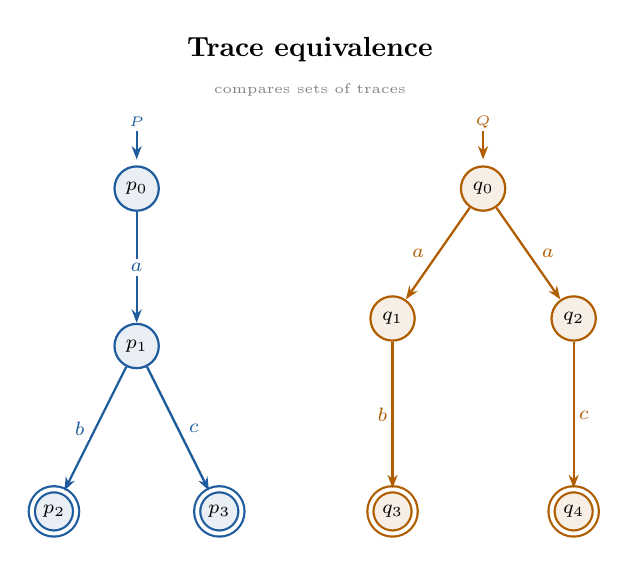
\begin{tikzpicture}
		
		%% ================================================================
		%% PANEL A  ·  Trace Equivalence
		%%
		%%   P = a.(b.0 + c.0)          (one a-step, then nondeterministic)
		%%   Q = a.b.0 + a.c.0          (two a-branches, each deterministic)
		%%   Both have  T(P) = T(Q) = {ε, a, ab, ac}
		%%
		%% x range : 0 – 7.2
		%% ================================================================
		\node[ht] at (3.6,.82){Trace equivalence};
		\node[hs] at (3.6,.30){compares sets of traces};
		
		%% process P
		\node[font=\tiny\bfseries,CB] at (1.4,-.10){$P$};
		\draw[tr=CB](1.4,-.22)--(1.4,-.58);
		\node[nd=CB] (p0) at (1.4,-.95){$p_0$};
		\node[nd=CB] (p1) at (1.4,-2.95){$p_1$};
		\node[ndf=CB](p2) at (.35,-5.05){$p_2$};
		\node[ndf=CB](p3) at (2.45,-5.05){$p_3$};
		\draw[tr=CB](p0)--node[el]{$a$}(p1);
		\draw[tr=CB](p1)--node[el,left=2pt]{$b$}(p2);
		\draw[tr=CB](p1)--node[el,right=2pt]{$c$}(p3);
		
		%% process Q
		\node[font=\tiny\bfseries,CO] at (5.8,-.10){$Q$};
		\draw[tr=CO](5.8,-.22)--(5.8,-.58);
		\node[nd=CO] (q0) at (5.8,-.95){$q_0$};
		\node[nd=CO] (q1) at (4.65,-2.60){$q_1$};
		\node[nd=CO] (q2) at (6.95,-2.60){$q_2$};
		\node[ndf=CO](q3) at (4.65,-5.05){$q_3$};
		\node[ndf=CO](q4) at (6.95,-5.05){$q_4$};
		\draw[tr=CO](q0)--node[el,left=3pt]{$a$}(q1);
		\draw[tr=CO](q0)--node[el,right=3pt]{$a$}(q2);
		\draw[tr=CO](q1)--node[el,left]{$b$}(q3);
		\draw[tr=CO](q2)--node[el,right]{$c$}(q4);
		
		%% result
%		\node[rb] at (3.6,-6.05)
%		{$\mathcal{T}(P)=\mathcal{T}(Q)=\{a,\,ab,\,ac, \varepsilon\}$};
%		\node[hs,color=CG] at (3.6,-6.70)
%		{$P \approx_{\mathrm{tr}} Q$ \enspace — same observable sequences};
%		
%		%% not bisimilar footnote
%		\node[hs] at (3.6,-7.20)
%		{\textit{(but not bisimilar: branching structure differs)}};
		
%		%% ================================================================
%		%% PANEL B  ·  Open Bisimilarity
%		%%
%		%%   P sends name $x$ on channel $a$, then receives on $b$
%		%%   Q sends name $y$ on channel $a$, then receives on $b$
%		%%   Bisim relation R closed under all name substitutions σ
%		%%
%		%% x-offset = 8.8
%		%% ================================================================
%		\def\bx{8.8}
%		
%		\node[ht] at (\bx+3.4,.82){Open bisimilarity};
%		\node[hs] at (\bx+3.4,.30){compares processes step by step};
%		
%		%% process P
%		\node[font=\tiny\bfseries,CB] at (\bx+1.2,-.10){$P$};
%		\draw[tr=CB](\bx+1.2,-.22)--(\bx+1.2,-.58);
%		\node[nd=CB] (bp0) at (\bx+1.2,-.95) {$p_0$};
%		\node[nd=CB] (bp1) at (\bx+1.2,-3.05){$p_1$};
%		\node[ndf=CB](bp2) at (\bx+1.2,-5.15){$p_2$};
%		\draw[tr=CB](bp0)--node[el,left]{$\bar{a}\langle x\rangle$}(bp1);
%		\draw[tr=CB](bp1)--node[el,left]{$b(z)$}(bp2);
%		
%		%% process Q
%		\node[font=\tiny\bfseries,CO] at (\bx+5.6,-.10){$Q$};
%		\draw[tr=CO](\bx+5.6,-.22)--(\bx+5.6,-.58);
%		\node[nd=CO] (bq0) at (\bx+5.6,-.95) {$q_0$};
%		\node[nd=CO] (bq1) at (\bx+5.6,-3.05){$q_1$};
%		\node[ndf=CO](bq2) at (\bx+5.6,-5.15){$q_2$};
%		\draw[tr=CO](bq0)--node[el,right]{$\bar{a}\langle y\rangle$}(bq1);
%		\draw[tr=CO](bq1)--node[el,right]{$b(w)$}(bq2);
%		
%		%% bisimulation relation at each level
%		\draw[rel](bp0)--node[el]{$\mathcal{R}$}(bq0);
%		\draw[rel](bp1)--node[el]{$\mathcal{R}\,[x{=}y]$}(bq1);
%		\draw[rel](bp2)--node[el]{$\mathcal{R}\,[z{=}w]$}(bq2);
%		
%		%% step annotations
%		\node[hs] at (\bx+3.4,-2.0){\textit{step 1 — match output, unify names}};
%		\node[hs] at (\bx+3.4,-4.1){\textit{step 2 — match input, bind names}};
%		
%		%% result
%		\node[rb] at (\bx+3.4,-6.05)
%		{$P\sim^{\!o}Q$ \enspace for all substitutions $\sigma$};
%		\node[hs,color=CG] at (\bx+3.4,-6.70)
%		{names unified; frames matched at each step};
%		\node[hs] at (\bx+3.4,-7.20)
%		{\textit{(stronger than trace eq.; closed under name instantiation)}};
%		
%		%% ================================================================
%		%% PANEL C  ·  Diff-Equivalence
%		%%
%		%%   Biprocess  B  has two diff-transitions:
%		%%       s0 –diff(m,n)→ s1 –diff(p,q)→ s2 –c→ s3
%		%%   Left  projection π₁ : m, p, c
%		%%   Right projection π₂ : n, q, c     ← same control flow
%		%%
%		%% x-offset = 17.6
%		%% ================================================================
%		\def\cx{17.6}
%		
%		\node[ht] at (\cx+3.2,.82){Diff-equivalence};
%		\node[hs] at (\cx+3.2,.30){two synchronized projections of one biprocess};
%		
%		%% biprocess B  (compact – only 4 states needed)
%		\node[font=\tiny\bfseries,CP] at (\cx+3.2,-.10){$\mathcal{B}$};
%		\draw[tr=CP](\cx+3.2,-.22)--(\cx+3.2,-.58);
%		\node[nd=CP] (d0) at (\cx+3.2,-.95){$s_0$};
%		\node[nd=CP] (d1) at (\cx+3.2,-2.05){$s_1$};
%		\node[nd=CP] (d2) at (\cx+3.2,-3.15){$s_2$};
%		\draw[tr=CP](d0)--node[el,right,font=\tiny]{$\mathrm{diff}(m,n)$}(d1);
%		\draw[tr=CP](d1)--node[el,right,font=\tiny]{$\mathrm{diff}(p,q)$}(d2);
%		
%		%% projection arrows diverging from d2
%		\draw[pja=CT](d2)--(\cx+0.95,-4.12);
%		\node[font=\tiny,CT] at (\cx+1.85,-3.76){$\pi_1$};
%		\draw[pja=CR](d2)--(\cx+5.45,-4.12);
%		\node[font=\tiny,CR] at (\cx+4.55,-3.76){$\pi_2$};
%		
%		%% left projection  π₁(B)
%		\node[font=\tiny\bfseries,CT] at (\cx+0.95,-4.00){$\pi_1(\mathcal{B})$};
%		\node[nd=CT] (l0) at (\cx+0.95,-4.55){$s_0$};
%		\node[nd=CT] (l1) at (\cx+0.95,-5.75){$s_1$};
%		\node[nd=CT] (l2) at (\cx+0.95,-6.95){$s_2$};
%		\node[ndf=CT](l3) at (\cx+0.95,-8.15){$s_3$};
%		\draw[tr=CT](l0)--node[el,left]{$m$}(l1);
%		\draw[tr=CT](l1)--node[el,left]{$p$}(l2);
%		\draw[tr=CT](l2)--node[el,left]{$c$}(l3);
%		
%		%% right projection  π₂(B)
%		\node[font=\tiny\bfseries,CR] at (\cx+5.45,-4.00){$\pi_2(\mathcal{B})$};
%		\node[nd=CR] (r0) at (\cx+5.45,-4.55){$s_0$};
%		\node[nd=CR] (r1) at (\cx+5.45,-5.75){$s_1$};
%		\node[nd=CR] (r2) at (\cx+5.45,-6.95){$s_2$};
%		\node[ndf=CR](r3) at (\cx+5.45,-8.15){$s_3$};
%		\draw[tr=CR](r0)--node[el,right]{$n$}(r1);
%		\draw[tr=CR](r1)--node[el,right]{$q$}(r2);
%		\draw[tr=CR](r2)--node[el,right]{$c$}(r3);
%		
%		%% synchrony connectors (same state reached at each step)
%		\draw[dashed,gray!40,line width=0.55pt](l0)--(r0)
%		node[midway,hs,fill=white,inner sep=1pt]{same};
%		\draw[dashed,gray!40,line width=0.55pt](l1)--(r1)
%		node[midway,hs,fill=white,inner sep=1pt]{same};
%		\draw[dashed,gray!40,line width=0.55pt](l2)--(r2)
%		node[midway,hs,fill=white,inner sep=1pt]{same};
%		\draw[dashed,gray!40,line width=0.55pt](l3)--(r3)
%		node[midway,hs,fill=white,inner sep=1pt]{same};
%		
%		%% result
%		\node[rb] at (\cx+3.2,-9.00)
%		{$\mathcal{B}$ diff-equiv $\;\Leftrightarrow\;
%			\pi_1(\mathcal{B})\approx\pi_2(\mathcal{B})$};
%		\node[hs,color=CG] at (\cx+3.2,-9.65)
%		{same control flow; only \texttt{diff}-terms differ};
%		
%		%% ================================================================
%		%% Vertical panel separators
%		%% ================================================================
%		\draw[gray!22,line width=0.7pt](8.0, 1.05)--(8.0,-10.0);
%		\draw[gray!22,line width=0.7pt](17.0,1.05)--(17.0,-10.0);
	\end{tikzpicture}
\end{document}